\section{Đề xuất kiến trúc phần mềm}
\label{sec:architecture}

Mục này được trình bày theo hai tầng. Trước hết là \emph{mô hình chung}
(Mục~\ref{sec:common}): những gì đúng với mọi bệnh viện, gồm các thành phần,
luồng xử lý một ca chụp, yêu cầu lưu trữ bền và cách phân tầng dữ liệu giữa
kho tại chỗ, kho ngoài cơ sở và kho lưu trữ lạnh. Sau đó mô hình chung được áp
vào \emph{tình hình cụ thể} của từng mẫu bối cảnh ở Mục~\ref{sec:contexts}
(Mục~\ref{sec:percontext}), và cuối cùng được mở rộng thành mô hình liên viện
(Mục~\ref{sec:hub}).

\subsection{Nguyên tắc thiết kế}

Năm nguyên tắc, rút ra từ các phân tích ở trên, chi phối cả ba kiến trúc.

\textbf{P1 --- Luồng xử lý hậu kỳ nằm ngoài đường tới hạn.} Việc chuyển ảnh tới
kho lưu trữ và tới trình xem không được phụ thuộc vào bất kỳ thành phần xử lý bổ
sung nào. Các tác vụ hậu kỳ được kích hoạt bởi một sự kiện phát ra \emph{sau}
khi ảnh đã được lưu an toàn, nhờ đó sự cố của chúng chỉ làm hệ thống suy giảm về
mức một PACS thông thường chứ không làm gián đoạn hoạt động khám chữa bệnh.

\textbf{P2 --- Lõi dùng chung, ngoại vi thay đổi.} Ba kiến trúc là các cấu hình
của cùng một tập thành phần, không phải ba hệ thống riêng biệt. Điều này giới
hạn công sức bảo trì và cho phép một cơ sở chuyển đổi giữa các bối cảnh khi hạ
tầng của họ được nâng cấp.

\textbf{P3 --- Dữ liệu mặc định ở lại nội bộ.} Theo yêu cầu L1, cấu hình triển
khai mặc định giữ toàn bộ dữ liệu và mọi xử lý bên trong cơ sở y tế. Việc đưa dữ
liệu ra ngoài phạm vi bệnh viện là một cấu hình tường minh, cần được biện minh
riêng.

\textbf{P4 --- Hệ thống hỗ trợ, không thay thế chuyên môn.} Nền tảng cung cấp
thông tin phục vụ chẩn đoán nhưng không đưa ra kết luận chẩn đoán. Mọi dữ liệu
do hệ thống sinh ra đều phải truy được nguồn gốc, có thể xem xét lại và không
bao giờ được ghi vào hồ sơ bệnh án nếu không có thao tác của bác sĩ.

\textbf{P5 --- Đã xác nhận là không được mất.} Khi cổng DICOM đã trả lời thành
công cho một lệnh C-STORE, thiết bị chụp được phép xoá bản của nó; từ thời điểm
đó nền tảng là nơi duy nhất giữ ca chụp. Vì vậy mọi đối tượng đã được xác nhận
phải tồn tại qua bất kỳ sự cố đơn lẻ nào của phần cứng, phần mềm hay đường
truyền (Mục~\ref{sec:durability}).

\subsection{Mô hình chung}
\label{sec:common}

\subsubsection{Các thành phần}

\begin{figure}[H]
\centering
\begin{tikzpicture}[
    node distance=1.1cm and 2.4cm,
    box/.style={draw, rounded corners=2pt, minimum width=2.5cm, minimum height=0.85cm,
                align=center, font=\small},
    aux/.style={box, fill=blue!8},
    stor/.style={box, fill=green!8},
    flow/.style={->, >=stealth, thick},
    evt/.style={->, >=stealth, thick, dashed}
]
\node[box] (mod) {Máy chụp CT};
\node[box, right=of mod] (gw) {Cổng DICOM\\\scriptsize(Orthanc)};
\node[box, right=of gw] (view) {Trình xem web\\\scriptsize(OHIF)};
\node[stor, below=of mod] (hot) {Kho ảnh tại chỗ\\\scriptsize(tầng nóng/ấm)};
\node[aux, below=of gw] (orch) {Bộ điều phối};
\node[aux, below=of orch] (task) {Dịch vụ xử lý\\hậu kỳ};
\node[box, right=of task] (store) {Kho siêu dữ liệu\\+ nhật ký truy vết};
\node[stor, below=of hot] (queue) {Hàng đợi đồng bộ\\\scriptsize(bền vững, trên đĩa)};
\node[stor, below=of queue, fill=gray!12] (off) {Kho ngoài cơ sở\\\scriptsize(sao lưu, lưu trữ lạnh)};

\draw[flow] (mod) -- node[above,font=\scriptsize] {C-STORE} (gw);
\draw[flow] (gw) -- node[above,font=\scriptsize] {DICOMweb} (view);
\draw[flow] (gw) -- node[pos=0.4,above,font=\scriptsize,sloped] {ghi rồi mới ACK} (hot);
\draw[evt] (gw) -- node[right,font=\scriptsize] {sự kiện} (orch);
\draw[flow] (orch) -- node[right,font=\scriptsize] {đã khử định danh} (task);
\draw[flow] (task) -- (store);
\draw[flow] (store.east) -- ++(0.7,0) |- (view.east);
\draw[evt] (orch) -- node[above,font=\scriptsize,sloped] {xếp hàng} (queue);
\draw[evt] (queue) -- node[right,font=\scriptsize] {bất đồng bộ, thử lại} (off);
\end{tikzpicture}
\caption{Mô hình thành phần dùng chung. Luồng nét liền từ máy chụp tới kho tại chỗ
và trình xem độc lập với các luồng nét đứt tới xử lý hậu kỳ và tới kho ngoài cơ
sở, hiện thực hoá nguyên tắc~P1.}
\label{fig:common}
\end{figure}

\begin{description}[leftmargin=3.2cm,style=nextline]
\item[Cổng DICOM] Tiếp nhận ca chụp qua C-STORE, ghi bền xuống kho tại chỗ rồi
      mới xác nhận, và cung cấp lại qua DICOMweb. Phát ra một sự kiện khi ảnh
      đến. Orthanc đảm nhiệm vai trò này, với cơ chế callback Lua trên sự kiện
      lưu đối tượng ảnh cung cấp sẵn cơ chế phát sự kiện \cite{jodogne2018orthanc}.
\item[Kho ảnh tại chỗ] Nơi giữ bản gốc còn định danh. Dữ liệu điểm ảnh được lưu
      dưới dạng tệp DICOM nguyên vẹn (có thể nén không mất mát,
      Mục~\ref{sec:transfersyntax}), trên đĩa cục bộ hoặc trên kho đối tượng
      tương thích S3 thông qua plugin lưu trữ đối tượng của Orthanc
      \cite{orthancbook}.
\item[Bộ điều phối] Tiêu thụ sự kiện ảnh đến, lọc theo loại thiết bị và vùng
      giải phẫu, khử định danh theo Mục~\ref{sec:deid}, ghép các đối tượng
      ảnh thành một ca chụp hoàn chỉnh, chuyển tới các tác vụ hậu kỳ và đưa
      các bản cần gửi ra ngoài vào hàng đợi đồng bộ. Bộ điều phối nắm giữ
      logic thử lại và kiểm soát tải, và là thành phần giữ cho các lỗi không
      lan rộng.
\item[Dịch vụ xử lý hậu kỳ] Thực hiện các tác vụ không nằm trên đường tới
      hạn, chẳng hạn trích xuất siêu dữ liệu, kiểm tra tính toàn vẹn của
      chuỗi ảnh, sinh ảnh thu nhỏ phục vụ duyệt nhanh, và chuẩn bị gói dữ
      liệu cho việc đọc từ xa. Dịch vụ này phi trạng thái, do đó có thể mở
      rộng theo chiều ngang. Đây cũng là điểm mở rộng dành cho các thành
      phần phân tích ảnh tự động trong các giai đoạn sau.
\item[Kho siêu dữ liệu và nhật ký truy vết] Lưu chỉ mục ca chụp theo khoá là
      UID kèm dấu thời gian, vị trí và tầng lưu trữ hiện tại của từng ca,
      tổng kiểm tra (checksum) của từng đối tượng, cùng với nhật ký truy cập
      chỉ ghi thêm theo yêu cầu L4. Kho này tách khỏi dữ liệu điểm ảnh; với
      Orthanc, chỉ mục có thể đặt trên PostgreSQL thay cho SQLite mặc định.
\item[Hàng đợi đồng bộ] Hàng đợi bền vững nằm trên đĩa cục bộ, chứa các bản
      cần gửi ra ngoài cơ sở. Phần tử chỉ bị xoá sau khi phía nhận xác nhận đã
      lưu và tổng kiểm tra khớp.
\item[Kho ngoài cơ sở] Nhận bản sao lưu đã mã hoá và, nếu được bật, bản đã khử
      định danh phục vụ đọc từ xa hay nghiên cứu. Đặt trong lãnh thổ Việt Nam
      theo L1.
\item[Trình xem] Hiển thị ảnh cho bác sĩ. OHIF đảm nhiệm vai trò này
      \cite{ziegler2020ohif}.
\end{description}

\subsubsection{Luồng xử lý chung của một ca chụp}
\label{sec:flow}

Luồng dưới đây giống nhau ở mọi bối cảnh; các bối cảnh chỉ khác nhau ở chỗ bước
nào được bật và mỗi kho được đặt ở đâu.

\begin{figure}[H]
\centering
\begin{tikzpicture}[
    node distance=0.55cm,
    stepbox/.style={draw, rounded corners=2pt, minimum width=11cm, minimum height=0.7cm,
                 align=left, font=\small, inner xsep=8pt},
    local/.style={stepbox, fill=green!6},
    cloudy/.style={stepbox, fill=blue!6},
    gate/.style={draw, diamond, aspect=3.4, inner sep=1pt, font=\scriptsize, align=center},
    arr/.style={->, >=stealth, thick}
]
\node[local] (s1) {\textbf{B1.} Thiết bị chụp gửi ảnh qua C-STORE tới cổng DICOM};
\node[local, below=of s1] (s2) {\textbf{B2.} Ghi bền xuống kho tại chỗ, tính checksum, rồi mới xác nhận cho thiết bị};
\node[local, below=of s2] (s3) {\textbf{B3.} Phát sự kiện ``ảnh đã đến'' tới bộ điều phối};
\node[local, below=of s3] (s4) {\textbf{B4.} Bác sĩ đã có thể đọc ảnh trên trình xem};
\node[local, below=of s4] (s5) {\textbf{B5.} Ghép đủ chuỗi ảnh, khử định danh, xử lý hậu kỳ};
\node[local, below=of s5] (s6) {\textbf{B6.} Lưu siêu dữ liệu, ghi nhật ký truy vết};
\node[gate, below=of s6, yshift=-0.12cm] (g) {Có cấu hình đích\\ngoài cơ sở?};
\node[cloudy, below=of g, yshift=-0.12cm] (s7) {\textbf{B7.} Đưa bản sao lưu mã hoá và (nếu bật) bản đã khử định danh vào hàng đợi};
\node[cloudy, below=of s7] (s8) {\textbf{B8.} Tiến trình nền gửi dần, thử lại khi lỗi, đối chiếu checksum rồi mới xoá};
\node[local, below=of s8] (s9) {\textbf{B9.} Vòng đời: chuyển tầng theo tuổi, nạp trước ca cũ, xoá khi hết hạn};

\foreach \a/\b in {s1/s2, s2/s3, s3/s4, s4/s5, s5/s6, s6/g, g/s7, s7/s8, s8/s9}
    \draw[arr] (\a) -- (\b);
\draw[arr] (g.east) -- node[above,font=\scriptsize] {không} (g.east -| s8.east) -- ++(0.6,0) |- (s9.east);
\end{tikzpicture}
\caption{Luồng xử lý chung của một ca chụp. Các bước nền xanh lá diễn ra hoàn toàn
trong mạng nội bộ bệnh viện; chỉ hai bước nền xanh dương liên quan tới kho ngoài
cơ sở, và chúng nằm sau thời điểm bác sĩ đã đọc được ảnh.}
\label{fig:flow}
\end{figure}

Diễn giải từng bước:

\begin{description}[leftmargin=1.4cm,style=nextline]
\item[B1] Thiết bị chụp mở một liên kết DICOM tới cổng DICOM và gửi từng lát
      cắt bằng lệnh C-STORE. Đây là cấu hình duy nhất cần thay đổi trên thiết
      bị chụp khi lắp đặt hệ thống.
\item[B2] Cổng DICOM ghi từng đối tượng ảnh xuống kho lưu trữ tại chỗ, tính và
      lưu tổng kiểm tra, rồi mới trả mã xác nhận thành công cho thiết bị chụp.
      Thứ tự này là hiện thực của nguyên tắc P5: chỉ khi dữ liệu đã nằm bền
      trên đĩa thì phía gửi mới được phép coi là đã gửi xong. Nếu cổng DICOM
      lỗi trước khi xác nhận, thiết bị chụp vẫn giữ bản của nó và gửi lại;
      trách nhiệm giữ dữ liệu vì thế không bao giờ bị ``rơi'' giữa hai bên.
\item[B3] Sau khi ghi xong, cổng DICOM phát một sự kiện nội bộ báo có ảnh
      mới. Trong bản mẫu, cơ chế này được hiện thực bằng callback Lua của
      Orthanc gọi tới bộ điều phối. Sự kiện được phát theo kiểu ``bắn và
      quên'': nếu bộ điều phối không phản hồi, cổng DICOM vẫn tiếp tục nhận
      các ảnh tiếp theo bình thường.
\item[B4] Ngay tại thời điểm này, trước khi bất kỳ xử lý hậu kỳ nào diễn ra,
      bác sĩ đã có thể mở trình xem và đọc ca chụp qua DICOMweb. Đây chính là
      biểu hiện cụ thể của nguyên tắc P1: giá trị lâm sàng cơ bản của hệ
      thống, tức việc xem được ảnh, không phụ thuộc vào các thành phần phụ
      trợ.
\item[B5] Bộ điều phối chờ cho tới khi nhận đủ số lát cắt của một chuỗi ảnh,
      lọc theo loại thiết bị và vùng giải phẫu, thực hiện khử định danh theo
      Mục~\ref{sec:deid}, rồi chuyển dữ liệu đã khử định danh tới dịch vụ xử
      lý hậu kỳ. Toàn bộ quá trình này chạy trong mạng nội bộ, không ra ngoài
      Internet.
\item[B6] Siêu dữ liệu được ghi vào kho kèm dấu thời gian, đồng thời một bản
      ghi được thêm vào nhật ký truy vết chỉ ghi thêm theo yêu cầu L4.
\item[B7] Nếu cơ sở đã cấu hình đích ngoài cơ sở, hai loại bản sao được đưa vào
      hàng đợi bền vững trên đĩa cục bộ: \emph{bản sao lưu} của bản gốc, được
      mã hoá bằng khoá do bệnh viện nắm giữ trước khi rời máy chủ, và, nếu
      chức năng chia sẻ được bật, \emph{bản đã khử định danh}. Bản gốc ở dạng
      rõ không bao giờ đi vào hàng đợi này.
\item[B8] Một tiến trình nền lấy từng phần tử khỏi hàng đợi và gửi đi, sử dụng
      cơ chế thử lại với khoảng chờ tăng dần khi gặp lỗi mạng. Phần tử chỉ bị
      xoá khỏi hàng đợi sau khi phía nhận xác nhận đã lưu thành công và tổng
      kiểm tra khớp. Nhờ vậy, mất kết nối chỉ làm hàng đợi dài thêm chứ không
      gây mất dữ liệu.
\item[B9] Độc lập với B7--B8, chính sách vòng đời định kỳ chuyển các ca chụp
      cũ xuống tầng thấp hơn, nạp trước các ca cũ của một bệnh nhân vừa có chỉ
      định mới lên tầng nóng, và xoá có căn cứ khi hết thời hạn lưu trữ theo
      L6 (Mục~\ref{sec:tiering}).
\end{description}

\subsubsection{Nguyên tắc ghi cục bộ trước}
\label{sec:localfirst}

Cả ba kiến trúc đều tuân theo một nguyên tắc lưu trữ chung: ảnh chụp luôn được
ghi xuống kho cục bộ tại bệnh viện trước, và chỉ sau khi việc ghi đó hoàn tất
thì dữ liệu mới được cân nhắc gửi ra ngoài cơ sở. Đây không phải lựa chọn tuỳ
tiện mà là hệ quả bắt buộc của bốn ràng buộc đã phân tích ở các mục trước.

\textbf{Thứ nhất, ràng buộc pháp lý.} Theo yêu cầu L1 rút ra từ
Mục~\ref{sec:legal}, dữ liệu hình ảnh còn định danh phải nằm trong phạm vi bệnh
viện, hoặc ít nhất trong lãnh thổ Việt Nam. Luật Bảo vệ dữ liệu cá nhân yêu cầu
lập và gửi hồ sơ đánh giá tác động khi chuyển dữ liệu cá nhân xuyên biên giới
\cite{pdpl2025}. Nếu hệ thống gửi thẳng ảnh lên một dịch vụ đám mây đặt ngoài
lãnh thổ trước khi lưu cục bộ thì hành vi chuyển dữ liệu đã xảy ra ngay tại thời
điểm đó và không thể thu hồi. Ghi cục bộ trước bảo đảm luôn tồn tại một bản gốc
hợp pháp nằm trong tầm kiểm soát của bệnh viện, còn việc đưa dữ liệu ra ngoài
trở thành một quyết định tách rời, có thể kiểm soát, có thể từ chối và có thể
ghi nhật ký.

\textbf{Thứ hai, an toàn lâm sàng.} Theo nguyên tắc P1, các tác vụ phụ trợ không
được nằm trên đường tới hạn của việc chuyển ảnh tới bác sĩ. Nếu bước ghi dữ liệu
phụ thuộc vào kết nối Internet thì một sự cố đường truyền sẽ chặn đứng cả việc
lưu ảnh lẫn việc đọc ảnh, biến một sự cố hạ tầng thông thường thành một sự cố an
toàn người bệnh. Kho cục bộ đóng vai trò điểm cam kết dữ liệu: sau khi ảnh được
ghi thành công xuống đĩa tại chỗ, ca chụp đã an toàn và bác sĩ có thể đọc được,
bất kể mọi thành phần phía sau có hoạt động hay không.

\textbf{Thứ ba, đặc tính của đường truyền.} Một ca chụp CT sọ não thường gồm vài
trăm lát cắt với dung lượng từ 100 đến 500~MB. Hình~\ref{fig:transfer} cho thấy
thời gian truyền một ca theo băng thông: trên mạng nội bộ 1~Gbps, việc ghi mất
vài giây; trên đường truyền 5~Mbps điển hình của một kết nối yếu ở bối cảnh C,
một ca 500~MB cần khoảng 19 phút, và vẫn cần khoảng 8 phút ngay cả khi đã nén
không mất mát. Truyền đồng bộ một khối dữ liệu như vậy dễ thất bại giữa chừng;
ghi cục bộ trước đẩy phần việc chậm và dễ lỗi này sang một tiến trình nền có khả
năng thử lại.

\begin{figure}[H]
\centering
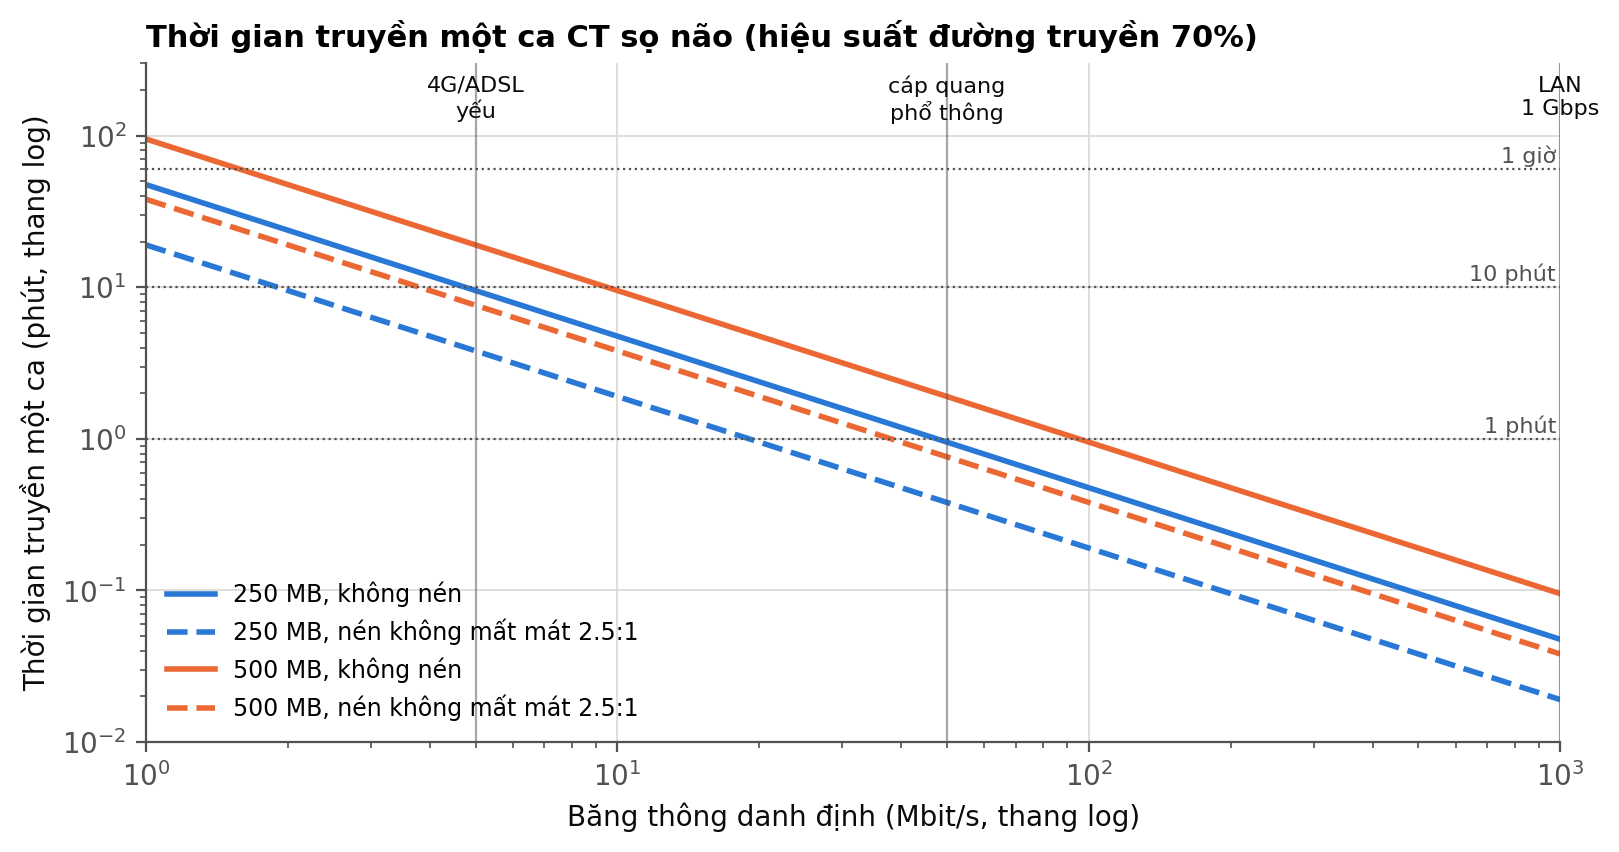
\includegraphics[width=0.88\textwidth]{figures/fig_transfer_time.png}
\caption{Ước lượng thời gian truyền một ca CT sọ não theo băng thông danh định, với
hiệu suất sử dụng đường truyền giả định 70\% và tỉ lệ nén không mất mát giả định
2{,}5:1 (nét đứt). Đây là ước lượng bậc độ lớn, không phải số đo. Mã nguồn:
\texttt{figures/src/fig\_transfer\_time.py}.}
\label{fig:transfer}
\end{figure}

\textbf{Thứ tư, tối thiểu hoá dữ liệu.} Theo yêu cầu L2, chỉ dữ liệu thực sự cần
thiết mới được truyền đi. Khử định danh và mã hoá là các bước xử lý cần thực
hiện trên bản gốc. Nếu dữ liệu được đẩy ra ngoài ngay khi vừa đến thì sẽ không
còn thời điểm nào để chèn các bước này vào giữa. Kho cục bộ tạo ra chính khoảng
thời gian đó.

\subsubsection{Yêu cầu lưu trữ bền}
\label{sec:durability}

Nguyên tắc P5 biến độ bền của kho lưu trữ thành yêu cầu chức năng. Cần phân biệt
bốn đại lượng: \emph{độ bền} (xác suất một đối tượng đã xác nhận không bị mất),
\emph{tính sẵn sàng} (tỉ lệ thời gian ảnh đọc được), \emph{RPO} (lượng dữ liệu tối
đa có thể mất, đo bằng thời gian) và \emph{RTO} (thời gian tối đa để khôi phục
dịch vụ). Một kho có thể sẵn sàng cao mà độ bền thấp, chẳng hạn một máy chủ chạy
ổn định trên một ổ đĩa duy nhất, và ngược lại. Nền tảng đạt độ bền bằng các cơ
chế chồng lớp sau, mỗi cơ chế chống lại một loại sự cố khác nhau.

\begin{enumerate}[label=D\arabic*.,leftmargin=1.2cm]
\item \textbf{Cam kết trước khi xác nhận.} Như bước B2: đối tượng được ghi
      xuống phương tiện bền và chỉ mục được cập nhật trước khi trả lời C-STORE.
      Cơ chế này chống mất dữ liệu trong khoảnh khắc chuyển giao giữa thiết bị
      chụp và nền tảng.
\item \textbf{Dự phòng phần cứng.} Trên một máy chủ đơn lẻ, đĩa được ghép
      RAID~1 hoặc RAID~6; trên cụm nhiều máy, kho đối tượng phân tán như Ceph
      \cite{weil2006ceph} hoặc MinIO nhân bản hay mã hoá xoá (erasure coding)
      dữ liệu qua nhiều nút. Cơ chế này chống hỏng đĩa hoặc hỏng một nút, nhưng
      \emph{không} phải là sao lưu: một lệnh xoá nhầm hay mã độc tống tiền sẽ
      được nhân bản ngay lập tức.
\item \textbf{Toàn vẹn.} Tổng kiểm tra của từng đối tượng được tính khi tiếp
      nhận và lưu trong chỉ mục; Orthanc hỗ trợ sẵn việc lưu MD5 cho mỗi tệp.
      Mỗi lần sao chép sang tầng khác hay ra ngoài cơ sở đều được đối chiếu
      tổng kiểm tra, và một tác vụ nền quét định kỳ toàn bộ kho để phát hiện
      hỏng dữ liệu âm thầm trên đĩa.
\item \textbf{Sao lưu theo quy tắc 3-2-1.} Ít nhất ba bản, trên hai loại
      phương tiện, trong đó một bản ở ngoài cơ sở. Bản ngoài cơ sở là bản sao
      lưu đã mã hoá ở bước B7, chống các sự cố mất toàn bộ địa điểm như cháy,
      ngập, trộm thiết bị.
\item \textbf{Bất biến.} Nhật ký truy vết và bản sao lưu ngoài cơ sở được ghi
      theo chế độ ghi một lần (WORM, hay khoá đối tượng trên kho tương thích
      S3) trong suốt thời hạn lưu trữ, để cả người vận hành lẫn mã độc đều
      không sửa hay xoá được trước hạn.
\item \textbf{Chỉ mục là dữ liệu dẫn xuất.} Vì mỗi tệp DICOM tự mô tả, mang
      đầy đủ siêu dữ liệu bên trong (Mục~\ref{sec:dicom}), kho điểm ảnh là
      nguồn dữ liệu gốc còn chỉ mục có thể dựng lại bằng cách quét lại kho. Chỉ
      mục vẫn được sao lưu (kèm nhật ký giao dịch nếu dùng PostgreSQL) để khôi
      phục nhanh, nhưng mất chỉ mục không đồng nghĩa với mất ảnh.
\item \textbf{Diễn tập khôi phục.} Việc khôi phục từ bản sao lưu được thực
      hiện thử định kỳ và đo thời gian; một bản sao lưu chưa từng được khôi phục
      thử thì chưa thể coi là bản sao lưu.
\end{enumerate}

\subsubsection{Phân tầng lưu trữ theo vòng đời}
\label{sec:tiering}

Tần suất truy cập ảnh y khoa giảm theo tuổi của ca chụp một cách khá dự đoán
được: cao trong vài tháng đầu cho việc đọc và tái khám, giảm mạnh sau 6--12 tháng
và hiếm khi được truy cập sau 2--3 năm \cite{awspacs2026}, trong khi thời hạn lưu
trữ hồ sơ bệnh án theo quy định kéo dài nhiều năm. Giữ toàn bộ dữ liệu trên
phương tiện đắt tiền nhất là lãng phí; ngược lại, đưa ca chụp của tuần trước
xuống kho lạnh sẽ làm hỏng trải nghiệm đọc ảnh. Nền tảng vì vậy chia kho thành
bốn tầng (Bảng~\ref{tab:tiers}, Hình~\ref{fig:tiers}).

\begin{table}[H]
\centering
\small
\begin{tabularx}{\textwidth}{@{}l Y Y Y p{2.3cm}@{}}
\toprule
\textbf{Tầng} & \textbf{Vị trí và phương tiện} & \textbf{Dữ liệu} & \textbf{Vai trò} & \textbf{Truy xuất} \\
\midrule
T0 -- Nóng & Tại chỗ; SSD hoặc HDD RAID gắn với cổng DICOM & Ca chụp đến 12 tháng tuổi và mọi ca đang được đọc hoặc vừa được nạp trước & Phục vụ đọc ảnh & mili giây \\
T1 -- Ấm & Tại chỗ; kho đối tượng tương thích S3 (MinIO, Ceph RGW) hoặc NAS dung lượng lớn & Ca chụp 1--3 năm tuổi & So sánh với ca cũ, tái khám & dưới 1 giây -- vài giây \\
T2 -- Ngoài cơ sở & Trung tâm dữ liệu tuyến trên hoặc đám mây đặt tại Việt Nam & Bản sao lưu mã hoá của mọi ca; bản đã khử định danh nếu bật chia sẻ & Sao lưu 3-2-1, đọc từ xa & giây -- phút qua WAN \\
T3 -- Lạnh & Ngoài cơ sở; lớp lưu trữ lạnh của kho đối tượng hoặc băng từ & Bản sao lưu của ca trên 3 năm tuổi & Lưu trữ tuân thủ thời hạn & giờ \\
\bottomrule
\end{tabularx}
\caption{Bốn tầng lưu trữ của nền tảng. Ngưỡng tuổi là giá trị mặc định, cấu hình
được theo từng cơ sở.}
\label{tab:tiers}
\end{table}

\begin{figure}[H]
\centering
\begin{tikzpicture}[
    tier/.style={draw, rounded corners=2pt, text width=7.0cm, minimum height=1.0cm,
                 align=left, font=\small, inner xsep=6pt},
    lat/.style={font=\scriptsize, align=left, text width=2.4cm},
    arr/.style={->, >=stealth, thick}
]
\node[tier, fill=red!8] (t0) {\textbf{T0 -- Nóng} (tại chỗ)\\\scriptsize SSD/HDD RAID gắn với cổng DICOM; ca $\le$ 12 tháng};
\node[tier, fill=orange!10, below=1.0cm of t0] (t1) {\textbf{T1 -- Ấm} (tại chỗ)\\\scriptsize kho đối tượng tương thích S3 hoặc NAS; 1--3 năm};
\node[tier, fill=blue!8, below=1.0cm of t1] (t2) {\textbf{T2 -- Ngoài cơ sở} (trong lãnh thổ Việt Nam)\\\scriptsize bản sao lưu mã hoá của mọi ca; bản khử định danh};
\node[tier, fill=gray!12, below=1.0cm of t2] (t3) {\textbf{T3 -- Lạnh} (ngoài cơ sở)\\\scriptsize lớp lưu trữ lạnh hoặc băng từ; $>$ 3 năm};
\node[lat, right=0.3cm of t0] {mili giây};
\node[lat, right=0.3cm of t1] {dưới 1 giây -- vài giây};
\node[lat, right=0.3cm of t2] {giây -- phút (qua WAN)};
\node[lat, right=0.3cm of t3] {giờ};
\draw[arr] ([xshift=-1.6cm]t0.south) -- node[left,font=\scriptsize] {chuyển tầng theo tuổi} ([xshift=-1.6cm]t1.north);
\draw[arr] ([xshift=1.6cm]t1.north) -- node[right,font=\scriptsize] {nạp trước ca cũ} ([xshift=1.6cm]t0.south);
\draw[arr, dashed] (t0.west) -- ++(-2.5,0) |- node[pos=0.25,left,font=\scriptsize,align=right] {sao chép\\bất đồng bộ\\(B7--B8)} (t2.west);
\draw[arr] ([xshift=-1.6cm]t2.south) -- node[left,font=\scriptsize] {chuyển tầng theo tuổi} ([xshift=-1.6cm]t3.north);
\end{tikzpicture}
\caption{Phân tầng lưu trữ. Hai tầng trên nằm tại bệnh viện và phục vụ đọc ảnh; hai
tầng dưới nằm ngoài cơ sở và phục vụ độ bền (quy tắc 3-2-1) cùng thời hạn lưu trữ.
Bên phải là thời gian truy xuất điển hình.}
\label{fig:tiers}
\end{figure}

Ba quyết định thiết kế đi kèm việc phân tầng:

\begin{itemize}
\item \textbf{Một giao diện lưu trữ cho mọi tầng.} Kho tương thích S3 được dùng
      cho cả T1 tại chỗ lẫn T2--T3 ngoài cơ sở, nên cổng DICOM chỉ cần một
      plugin lưu trữ đối tượng, và việc chuyển tầng trở thành chính sách vòng
      đời của kho chứ không phải mã nguồn riêng. Điều này phù hợp với P2: cùng
      một bản cài đặt, khác nhau ở cấu hình đích lưu trữ.
\item \textbf{Nạp trước theo chỉ định.} Khi HIS/RIS phát một chỉ định mới
      (Mục~\ref{sec:his}), bộ điều phối kéo các ca cũ của cùng bệnh nhân từ T1
      hoặc T2 lên T0 trước khi bệnh nhân được chụp, để bác sĩ so sánh được ngay
      khi ca mới đến. Đây là thực hành chuẩn của PACS và là lý do T1 phải
      truy xuất được trong vài giây chứ không phải vài giờ.
\item \textbf{Xoá có căn cứ.} Khi một ca hết thời hạn lưu trữ theo L6, việc xoá
      được thực hiện đồng thời ở mọi tầng, được ghi vào nhật ký truy vết, và
      không áp dụng cho các ca đang bị giữ lại vì lý do pháp lý.
\end{itemize}

Hình~\ref{fig:storage} ước lượng quy mô dữ liệu, chỉ tính riêng CT sọ não với
100~MB mỗi ca sau khi nén không mất mát. Một cơ sở bối cảnh A với khoảng 60 ca
mỗi ngày tích luỹ khoảng 2{,}2~TB mỗi năm, bối cảnh B với khoảng 30 ca mỗi ngày
khoảng 1{,}1~TB mỗi năm, và bối cảnh C với khoảng 5 ca mỗi ngày chỉ khoảng
0{,}18~TB mỗi năm. Điểm quan trọng là tầng nóng T0 \emph{không} tăng theo thời
gian: nó dừng ở mức một năm dữ liệu, trong khi toàn bộ phần tăng trưởng dồn vào
các tầng rẻ hơn. Toàn bộ khoa chẩn đoán hình ảnh, gồm các vùng chụp khác, MRI và
X-quang, sẽ lớn hơn nhiều lần; con số cần được tính lại theo thống kê thực tế của
từng cơ sở khi triển khai.

\begin{figure}[H]
\centering
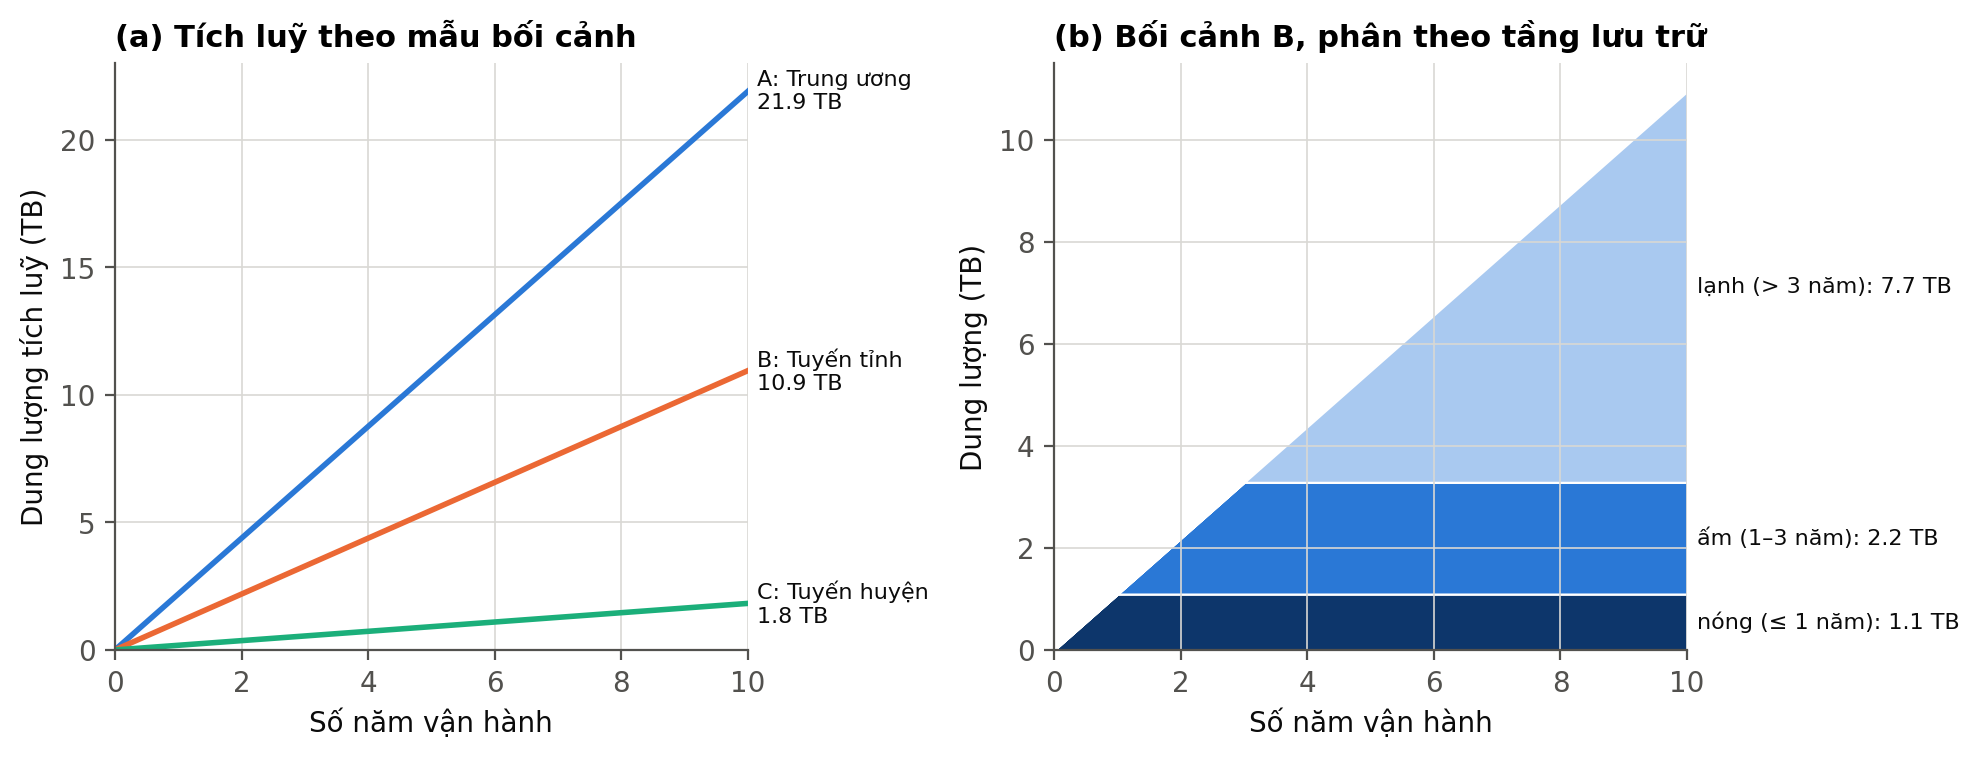
\includegraphics[width=\textwidth]{figures/fig_storage_growth.png}
\caption{Ước lượng dung lượng lưu trữ CT sọ não: (a) tích luỹ theo mẫu bối cảnh;
(b) bối cảnh B phân theo tầng lưu trữ. Giả định 250~MB/ca, nén không mất mát
2{,}5:1, ngưỡng tầng 1 và 3 năm. Mã nguồn: \texttt{figures/src/fig\_storage\_growth.py}.}
\label{fig:storage}
\end{figure}

\subsubsection{Vai trò của kho ngoài cơ sở}
\label{sec:offsite}

Kho ngoài cơ sở không tham gia vào việc cung cấp hình ảnh cho bác sĩ đọc tại
chỗ. Nó phục vụ ba mục đích, mỗi mục đích nhận một loại bản sao khác nhau:

\begin{enumerate}
\item \textbf{Sao lưu và lưu trữ dài hạn.} Nhận bản sao lưu của bản gốc, được
      mã hoá trước khi rời bệnh viện bằng khoá do bệnh viện quản lý, nên bên
      vận hành kho ngoài cơ sở chỉ giữ dữ liệu đã mã hoá. Để tránh hoàn toàn
      câu hỏi về chuyển dữ liệu xuyên biên giới, kho này được đặt trong lãnh
      thổ Việt Nam và được ràng buộc bằng hợp đồng xử lý dữ liệu.
\item \textbf{Chẩn đoán hình ảnh từ xa.} Nhận bản đã khử định danh để bác sĩ
      tuyến trên đọc (Mục~\ref{sec:percontext}, bối cảnh C). Bảng ánh xạ từ
      định danh giả về định danh thật chỉ nằm tại cơ sở gửi, nên kết quả đọc
      trả về được gắn lại đúng bệnh nhân tại chỗ.
\item \textbf{Tích luỹ dữ liệu phục vụ nghiên cứu.} Dữ liệu đã khử định danh
      kèm kết quả đọc của bác sĩ tạo thành tập dữ liệu phục vụ các nghiên cứu
      về sau. Theo yêu cầu L7, mục đích này phải có căn cứ pháp lý riêng,
      tách bạch với mục đích khám chữa bệnh.
\end{enumerate}

Không mục đích nào trong ba mục đích trên mang tính cấp thời, nên kho ngoài cơ sở
có thể ngừng hoạt động mà hệ thống vẫn phục vụ đầy đủ chức năng lâm sàng: đây là
thuộc tính thiết kế quan trọng nhất của mô hình lưu trữ này. Tuy nhiên, \emph{chức
năng} không phụ thuộc vào kho ngoài cơ sở không có nghĩa là \emph{độ bền} không phụ
thuộc: ở nơi chỉ có một máy chủ, bản sao lưu ngoài cơ sở là lớp bảo vệ duy nhất
trước sự cố mất toàn bộ địa điểm (D4).

\begin{table}[H]
\centering
\small
\begin{tabularx}{\textwidth}{@{}l Y Y Y@{}}
\toprule
\textbf{Tiêu chí} & \textbf{Kho tại chỗ (T0--T1)} & \textbf{Sao lưu ngoài cơ sở (T2--T3)} & \textbf{Bản chia sẻ (T2)} \\
\midrule
Dữ liệu & Bản gốc còn định danh & Bản gốc, đã mã hoá & Bản đã khử định danh \\
Tính bắt buộc & Bắt buộc & Khuyến nghị; bắt buộc nếu chỉ có một máy chủ & Tuỳ chọn, mặc định tắt \\
Thời điểm ghi & Đồng bộ, trước khi xác nhận & Bất đồng bộ, sau B6 & Bất đồng bộ, sau B6 \\
Khi mất mạng & Không ảnh hưởng & Hàng đợi dài thêm, không mất dữ liệu & Hàng đợi dài thêm \\
Vai trò trong đọc ảnh & Nguồn dữ liệu chính & Chỉ dùng khi khôi phục & Đọc từ xa \\
Ràng buộc pháp lý & Thuộc phạm vi bệnh viện & Đặt tại Việt Nam, hợp đồng xử lý dữ liệu & Khử định danh theo PS3.15; mục đích L7 \\
\bottomrule
\end{tabularx}
\caption{Phân vai giữa kho tại chỗ và hai loại bản sao ngoài cơ sở.}
\label{tab:localcloud}
\end{table}

\subsection{Áp dụng vào từng bối cảnh bệnh viện}
\label{sec:percontext}

Mỗi kiến trúc dưới đây là một cấu hình của mô hình chung, được mô tả theo cùng
một khung: hiện trạng của cơ sở, cách triển khai, cách hiện thực các tầng lưu
trữ, kết nối và đồng bộ, và hành vi khi có sự cố.

\subsubsection{Kiến trúc A: bệnh viện tuyến trung ương, tích hợp dạng đi kèm}

\textbf{Hiện trạng.} Cơ sở đã có PACS hoặc VNA thương mại vận hành ổn định, có
sao lưu, tích hợp với HIS/RIS qua HL7, có phòng CNTT và mạng nội bộ dự phòng.
Khối lượng trên 50 ca CT sọ não mỗi ngày, bác sĩ chẩn đoán hình ảnh trực 24/7.
Yêu cầu là không làm xáo trộn quy trình và không thay thế hệ thống sẵn có.

\textbf{Triển khai.} Cổng DICOM được triển khai không phải như kho lưu trữ mà
như một thành phần \emph{đi kèm} (sidecar): PACS được cấu hình để chuyển tiếp các
ca chụp CT sọ não tới nó bằng luật định tuyến C-STORE, và nền tảng ghi kết quả
xử lý ngược trở lại dưới dạng đối tượng DICOM Structured Report hoặc Secondary
Capture, hoặc thông qua giao diện danh sách chờ đọc của nhà cung cấp nếu có.
Để đáp ứng thông lượng, dịch vụ xử lý hậu kỳ phi trạng thái được nhân bản theo
chiều ngang, và nhiều phiên bản cổng DICOM dùng chung một chỉ mục PostgreSQL và
một kho đối tượng.

\textbf{Lưu trữ.} PACS sẵn có là nguồn dữ liệu gốc và tự đảm nhận T1--T3 cùng
sao lưu. Nền tảng chỉ giữ một bộ đệm T0 cuốn chiếu, chẳng hạn 90 ngày, tương
đương khoảng 0{,}55~TB với khối lượng trên, cộng với các kết quả do nó sinh ra;
các kết quả này được ghi ngược về PACS nên cũng được PACS lưu trữ dài hạn. Vì
vậy yêu cầu độ bền với nền tảng ở bối cảnh này nhẹ hơn hẳn: mất bộ đệm chỉ cần
lấy lại từ PACS bằng C-MOVE. Nguyên tắc chung là trách nhiệm về độ bền thuộc về
nơi giữ bản gốc.

\textbf{Kết nối.} Chỉ mạng nội bộ; không có đích ngoài cơ sở.

\textbf{Khi có sự cố.} Tính chất cốt yếu là gỡ bỏ nền tảng sẽ đưa bệnh viện trở
lại đúng trạng thái trước đó: không một thành phần sẵn có nào phụ thuộc vào nó.
Nếu nền tảng ngừng hoạt động, luật chuyển tiếp của PACS xếp hàng và gửi lại khi
nền tảng hoạt động trở lại.

\subsubsection{Kiến trúc B: bệnh viện tuyến tỉnh, triển khai tích hợp}

\textbf{Hiện trạng.} Có PACS nhưng có thể là sản phẩm đời cũ, dung lượng hạn
chế, hỗ trợ DICOMweb không chắc chắn. Có một đến hai nhân sự CNTT đa năng và một
số máy chủ; GPU chưa chắc có. Khối lượng 10--50 ca CT sọ não mỗi ngày; bác sĩ chẩn
đoán hình ảnh chỉ có mặt trong giờ hành chính. Đây là trường hợp phổ biến nhất và
là mục tiêu chính.

\textbf{Triển khai.} Nền tảng cung cấp cả cổng DICOM lẫn trình xem, hoạt động
song song với PACS. Khi PACS hỗ trợ DICOMweb, nền tảng đọc dữ liệu từ đó; khi
không, thiết bị chụp được cấu hình gửi đồng thời tới cả PACS và cổng DICOM, việc
trùng lặp này được ưu tiên hơn so với phụ thuộc vào một giao diện có thể không
hoạt động. Toàn bộ dịch vụ đóng gói container trên một đến hai máy chủ, đặt sau
reverse proxy đảm nhiệm kết thúc TLS và chuyển tiếp các yêu cầu DICOMweb. Đây là
cấu hình mà bản mẫu hiện tại hiện thực.

\textbf{Lưu trữ.} Nền tảng giữ bản gốc của riêng nó và hiện thực đủ bốn tầng.
T0 là mảng RAID trên máy chủ cổng DICOM, giữ khoảng một năm dữ liệu, tức cỡ
1{,}1~TB cho CT sọ não. T1 là kho đối tượng tương thích S3 tại chỗ, trên ba nút
trở lên nếu có đủ máy chủ, hoặc một NAS RAID~6 nếu không; sau mười năm, phần này
chứa phần lớn trong khoảng 11~TB tích luỹ (Hình~\ref{fig:storage}b). T2--T3 là
bản sao lưu mã hoá gửi tới trung tâm dữ liệu của tuyến trung ương hoặc một dịch
vụ đám mây đặt tại Việt Nam. Với chỉ một đến hai nhân sự CNTT, sao lưu, quét toàn
vẹn và diễn tập khôi phục phải được tự động hoá hoàn toàn và báo cáo qua giám sát
chứ không dựa vào thao tác thủ công.

\textbf{Kết nối.} Đọc ảnh trong giờ hành chính qua mạng nội bộ. Ngoài giờ, bác sĩ
trực từ xa truy cập trình xem qua VPN hoặc qua reverse proxy có xác thực; với
đường truyền 50~Mbps, một ca 250~MB cần khoảng một phút (Hình~\ref{fig:transfer}),
và cơ chế tải lũy tiến (Mục~\ref{sec:transfersyntax}) cho phép bắt đầu đọc sớm
hơn nữa. Cơ sở tuyến tỉnh cũng là ứng viên tự nhiên để làm trung tâm cho các cơ
sở tuyến huyện trong tỉnh (Mục~\ref{sec:hub}).

\textbf{Khi có sự cố.} Hỏng một đĩa: RAID che giấu, không gián đoạn. Hỏng máy chủ
cổng DICOM: PACS vẫn nhận ảnh nhờ gửi song song; nền tảng được dựng lại và khôi
phục từ T1 hoặc T2 trong vài giờ. Mất Internet: đọc tại chỗ không ảnh hưởng, chỉ
hàng đợi sao lưu dài thêm và đọc từ xa ngoài giờ bị gián đoạn.

\subsubsection{Kiến trúc C: bệnh viện tuyến huyện, thiết bị trọn gói}

\textbf{Hiện trạng.} Có máy CT nhưng không có PACS; hình ảnh nằm trên ổ cứng của
máy trạm thiết bị chụp, dung lượng có hạn và thường bị ghi đè khi đầy, nên rủi ro
mất ảnh là tình trạng sẵn có chứ không phải rủi ro mới. Không có phòng máy chủ,
không có nhân sự CNTT, không có bác sĩ chẩn đoán hình ảnh tại chỗ; nguồn điện và
kết nối mạng có thể không ổn định. Khối lượng dưới 10 ca CT sọ não mỗi ngày.

\textbf{Triển khai.} Nền tảng được chuyển giao dưới dạng một thiết bị trọn gói đã
cấu hình sẵn: một máy duy nhất, các dịch vụ đóng gói container, bộ lưu điện kèm
cơ chế tắt máy an toàn, quy trình lắp đặt chỉ gồm kết nối vật lý và một thay đổi
cấu hình trên thiết bị chụp. Cổng DICOM đóng luôn vai trò PACS của bệnh viện. Thiết
bị tự giám sát và gửi cảnh báo (đĩa, dung lượng, độ dài hàng đợi, nhiệt độ) tới đơn
vị hỗ trợ ở tuyến trên, vì tại chỗ không có ai đọc được bảng giám sát.

\textbf{Lưu trữ.} T0 và T1 gộp làm một trên thiết bị: hai ổ đĩa ghép RAID~1. Với
khoảng 0{,}18~TB CT sọ não mỗi năm, hai ổ vài TB đủ cho nhiều năm; con số cần được
tính lại theo tổng số ca của khoa. Vì chỉ có một thiết bị tại một địa điểm, bản sao
lưu mã hoá ngoài cơ sở (T2), đặt tại cơ sở tuyến tỉnh làm trung tâm, là lớp bảo vệ
duy nhất trước việc mất toàn bộ thiết bị; ở bối cảnh này nó là bắt buộc chứ không
còn là khuyến nghị.

\textbf{Kết nối và đồng bộ.} Toàn bộ chức năng tiếp nhận, lưu trữ và hiển thị chạy
cục bộ, nên mất kết nối không làm vô hiệu hoá hệ thống. Liên kết với tuyến trên là
\emph{theo cơ hội}: khi có kết nối, hàng đợi được giải phóng dần theo khả năng của
đường truyền. Trên đường truyền 5~Mbps, một ca 250~MB đã nén cần khoảng bốn phút
(Hình~\ref{fig:transfer}), nên hàng đợi cần phân mức ưu tiên: ca được đánh dấu
cần đọc từ xa đi trước, bản sao lưu đi sau và được giới hạn băng thông trong giờ
cao điểm. Bản gửi đọc từ xa là bản đã khử định danh; bảng ánh xạ định danh giả
nằm trên thiết bị, nên kết quả đọc trả về được gắn lại đúng bệnh nhân tại chỗ.

\textbf{Khi có sự cố.} Mất mạng: hàng đợi dài thêm, không mất dữ liệu. Hỏng một
đĩa: RAID~1 che giấu, thiết bị cảnh báo để thay đĩa. Mất điện: bộ lưu điện cho
phép tắt máy an toàn, và nhờ nguyên tắc P5 thiết bị chụp sẽ gửi lại các lát cắt
chưa được xác nhận. Mất toàn bộ thiết bị: thay thiết bị mới và khôi phục từ bản
sao lưu tại tuyến trên; RPO bằng độ trễ của hàng đợi sao lưu tại thời điểm sự cố.

Vì không có bác sĩ chẩn đoán hình ảnh tại chỗ, giá trị chính của cấu hình này nằm
ở hai điểm: không còn mất ảnh do máy trạm bị ghi đè, và rút ngắn thời gian đưa hình
ảnh tới người đọc có chuyên môn ở tuyến trên, thay vì chờ chuyển bệnh nhân hoặc
chuyển dữ liệu thủ công qua đĩa quang.

\subsubsection{So sánh}

\begin{table}[H]
\centering
\small
\begin{tabularx}{\textwidth}{@{}l Y Y Y@{}}
\toprule
& \textbf{A: Đi kèm} & \textbf{B: Tích hợp} & \textbf{C: Trọn gói} \\
\midrule
Nguồn dữ liệu gốc & PACS sẵn có & Nền tảng, song song PACS & Nền tảng \\
Tầng T0 & Bộ đệm cuốn chiếu $\sim$90 ngày & RAID trên máy chủ, $\sim$1 năm & RAID~1 trên thiết bị (gộp T0--T1) \\
Tầng T1 & Do PACS đảm nhận & Kho đối tượng S3 hoặc NAS tại chỗ & Gộp vào T0 \\
Tầng T2--T3 & Do PACS đảm nhận & Sao lưu mã hoá tới tuyến trên hoặc đám mây trong nước & Sao lưu mã hoá tới trung tâm tuyến tỉnh (bắt buộc) \\
Dung lượng CT sọ não & $\sim$2{,}2~TB/năm & $\sim$1{,}1~TB/năm & $\sim$0{,}18~TB/năm \\
Trình xem & Sẵn có & Nền tảng (OHIF) & Nền tảng (OHIF) \\
Trả kết quả & DICOM SR về PACS & Hiển thị trên trình xem & Trình xem + kết quả đọc từ xa \\
Phụ thuộc mạng & Chỉ mạng nội bộ & Mạng nội bộ; Internet cho đọc ngoài giờ & Chịu được mất kết nối \\
Hỏng máy chủ & Không ảnh hưởng lâm sàng & Khôi phục trong vài giờ từ T1/T2 & Thay thiết bị, khôi phục từ tuyến trên \\
Vai trò lâm sàng & Bổ trợ quy trình sẵn có & Hỗ trợ ngoài giờ & Lưu trữ an toàn, kết nối tuyến trên \\
\bottomrule
\end{tabularx}
\caption{So sánh ba kiến trúc được đề xuất.}
\label{tab:arch}
\end{table}

\subsection{Mở rộng liên viện: mô hình trục--nan}
\label{sec:hub}

Khi nhiều cơ sở tuyến huyện cùng gửi ca chụp lên một cơ sở tuyến trên, các kiến
trúc C riêng lẻ ghép lại thành mô hình trục--nan (hub-and-spoke), tương tự kiến
trúc PACS lai mà AWS đề xuất cho các mạng lưới nhiều bệnh viện \cite{awspacs2026}:
mỗi cơ sở giữ kho cục bộ và phục vụ đọc tại chỗ ở tốc độ mạng nội bộ, còn trung
tâm nhận bản sao bất đồng bộ và giữ một chỉ mục chung chỉ chứa siêu dữ liệu (ca
chụp nào đang nằm ở cơ sở nào, ở tầng nào, đã đồng bộ tới đâu), không chứa dữ liệu
điểm ảnh.

\begin{figure}[H]
\centering
\begin{tikzpicture}[
    site/.style={draw, rounded corners=2pt, align=center, font=\small,
                 minimum width=3.0cm, minimum height=1.1cm, fill=green!6},
    hubbox/.style={draw, rounded corners=3pt, align=left, font=\small,
                   fill=blue!6, text width=6.6cm, inner sep=6pt},
    arr/.style={->, >=stealth, thick},
    sync/.style={->, >=stealth, thick, dashed}
]
\node[hubbox] (hub) {\textbf{Trung tâm}: bệnh viện tuyến tỉnh hoặc trung tâm dữ liệu trong nước\\[2pt]
  \scriptsize $\bullet$ chỉ mục vị trí ca chụp (chỉ siêu dữ liệu)\\
  \scriptsize $\bullet$ kho sao lưu mã hoá (T2--T3) của các cơ sở\\
  \scriptsize $\bullet$ kho ca chụp đã khử định danh chờ đọc từ xa\\
  \scriptsize $\bullet$ trình xem cho bác sĩ đọc từ xa};
\node[site, fill=orange!8, above=1.1cm of hub] (a) {Bệnh viện tuyến trung ương\\\scriptsize hội chẩn khi cần};
\node[site, below left=1.5cm and 0.6cm of hub] (c1) {Cơ sở C$_1$\\\scriptsize thiết bị trọn gói};
\node[site, below=1.5cm of hub] (c2) {Cơ sở C$_2$\\\scriptsize thiết bị trọn gói};
\node[site, below right=1.5cm and 0.6cm of hub] (c3) {Cơ sở C$_3$\\\scriptsize thiết bị trọn gói};
\foreach \c in {c1, c2, c3} {
  \draw[sync] (\c) to[bend left=12] (hub);
  \draw[arr] (hub) to[bend left=12] (\c);
}
\draw[sync] (hub) -- node[right,font=\scriptsize] {ca cần hội chẩn} (a);
\end{tikzpicture}
\caption{Mô hình trục--nan. Nét đứt: dữ liệu đi lên, bất đồng bộ qua hàng đợi (bản sao
lưu mã hoá và bản đã khử định danh). Nét liền: kết quả đọc trả về cơ sở dưới dạng
DICOM SR và được gắn lại định danh tại chỗ.}
\label{fig:hubspoke}
\end{figure}

Mô hình này tiếp thu ba điểm từ kiến trúc tham chiếu của AWS: tách chỉ mục khỏi
điểm ảnh, sao chép bất đồng bộ không chặn luồng lâm sàng, và phân tầng lưu trữ tại
trung tâm theo vòng đời. Nó khác ở ba giả định. Thứ nhất, trung tâm đặt tại hạ tầng
trong nước, không đặt tại một vùng đám mây ở nước ngoài, theo L1. Thứ hai, kết nối
giữa cơ sở và trung tâm là đường Internet không ổn định chứ không phải kênh riêng,
nên mọi tương tác đều bất đồng bộ và cơ sở không bao giờ phải chờ trung tâm. Thứ ba,
trung tâm chỉ thấy bản sao lưu đã mã hoá và bản đã khử định danh; do đó nó chưa có
chỉ mục bệnh nhân chung (MPI) liên kết các ca của cùng một người ở nhiều cơ sở. Việc
liên kết đó đòi hỏi xử lý dữ liệu định danh ở trung tâm, chẳng hạn dựa trên số định
danh cá nhân khi hồ sơ bệnh án điện tử đã kết nối cơ sở dữ liệu quốc gia về dân cư,
và cần căn cứ pháp lý riêng; đây là câu hỏi mở cho các giai đoạn sau.

\subsection{Bản mẫu}

Một bản mẫu hiện thực Kiến trúc B đã được xây dựng nhằm kiểm chứng mô hình thành
phần. Bản mẫu gồm các dịch vụ đóng gói container: Orthanc mở cổng DICOM cổ điển
để nhận dữ liệu từ thiết bị chụp và DICOMweb cho trình xem; OHIF chạy sau một
reverse proxy chuyển tiếp \texttt{/dicom-web} và \texttt{/wado} tới Orthanc, nhờ
đó tránh được các vấn đề về cross-origin; và một dịch vụ xử lý hậu kỳ được gọi
bởi callback Lua của Orthanc kích hoạt khi đối tượng ảnh đến.

Bản mẫu xác nhận cơ chế kích hoạt theo sự kiện và hướng tích hợp với trình xem.
Nó \emph{chưa} sẵn sàng triển khai: xác thực bị tắt và kênh truyền chưa được mã
hoá. Mỗi điểm trong số đó tương ứng với một yêu cầu ở Mục~\ref{sec:legal} và
được lên lịch xử lý trong Giai đoạn~2, cùng với các tầng T1--T3, hàng đợi đồng bộ
và các cơ chế độ bền D3--D7.

\subsection{Kiến trúc an toàn thông tin}

Việc hiện thực các yêu cầu ở Mục~\ref{sec:legal} đòi hỏi: kết thúc TLS tại
reverse proxy, với DICOM cổ điển được giới hạn trong một phân đoạn mạng riêng
hoặc bọc trong đường hầm, và xác thực nút mạng theo hồ sơ IHE ATNA khi DICOM đi qua
mạng không tin cậy \cite{iheiti}; xác thực người dùng qua một máy chủ định danh
OpenID Connect như Keycloak, liên kết với hệ thống thư mục của bệnh viện nếu có,
và phân quyền cho Orthanc qua plugin phân quyền nâng cao cùng orthanc-auth-service
\cite{keycloak,orthancauth}, kèm phân tách vai trò giữa bác sĩ chẩn đoán hình ảnh,
bác sĩ chỉ định và quản trị viên; mã hoá khi lưu trữ cho cả kho ảnh lẫn kho siêu
dữ liệu, với khoá mã hoá bản sao lưu ngoài cơ sở do bệnh viện nắm giữ; nhật ký truy
vết chỉ ghi thêm cho mọi lượt truy cập, lưu giữ theo L6; và khử định danh áp dụng
tại ranh giới của bộ điều phối, để các thuộc tính định danh không bao giờ rời khỏi
phạm vi kiểm soát. Việc cho phép truy cập ẩn danh và truyền dữ liệu ở dạng rõ
trong bản mẫu là những tiện lợi phục vụ phát triển, và bị cấm khi triển khai thực
tế.
